%%%%%%%%%%%%%%%%%%%%%%%%%%%%%%%%%%%%%%%%%
% Stylish Article
% LaTeX Template
% Version 2.0 (13/4/14)
%
% This template has been downloaded from:
% http://www.LaTeXTemplates.com
%
% Original author:
% Mathias Legrand (legrand.mathias@gmail.com)
%
% License:
% CC BY-NC-SA 3.0 (http://creativecommons.org/licenses/by-nc-sa/3.0/)
%
%%%%%%%%%%%%%%%%%%%%%%%%%%%%%%%%%%%%%%%%%

%----------------------------------------------------------------------------------------
%	PACKAGES AND OTHER DOCUMENT CONFIGURATIONS
%----------------------------------------------------------------------------------------

\documentclass[fleqn,12pt,onecolumn]{ipcc} % Document font size and equations flushed left

\usepackage{lipsum} % Required to insert dummy text. To be removed otherwise
\usepackage{tikz} % good quality graphs
\usepackage{pgfplots}
\usetikzlibrary{pgfplots.groupplots}
\pgfplotsset{compat=newest}

%----------------------------------------------------------------------------------------
%	COLUMNS
%----------------------------------------------------------------------------------------

\setlength{\columnsep}{0.55cm} % Distance between the two columns of text
\setlength{\fboxrule}{0.75pt} % Width of the border around the abstract

%----------------------------------------------------------------------------------------
%	COLORS
%----------------------------------------------------------------------------------------

\definecolor{IrishGreen}{RGB}{0,0,90} % Color of the article title and sections
\definecolor{RoyalBlue}{RGB}{0,20,20} % Color of the boxes behind the abstract and headings

%----------------------------------------------------------------------------------------
%	HYPERLINKS
%----------------------------------------------------------------------------------------

\usepackage[colorlinks=true,bookmarks=true,plainpages=false,
linkcolor=IrishGreen, citecolor=IrishGreen, 
urlcolor=IrishGreen,pagebackref]{hyperref}%links in pdf
\usepackage[compress,numbers,comma]{natbib} %references
\usepackage{hypernat} %references
%----------------------------------------------------------------------------------------
%	ARTICLE INFORMATION
%----------------------------------------------------------------------------------------

\JournalInfo{Intel Parallel Computing Centres Report} % Journal information
\Archive{WIP} % Additional notes (e.g. copyright, DOI, review/research article)

\PaperTitle{Porting DL\_POLY to Xeon Phi} % Article title

\Authors{Alin M. Elena\textsuperscript{1}*, Christian Lalanne\textsuperscript{1}, Victor Gamayunov\textsuperscript{2}, Gilles Civario\textsuperscript{1}, Michael Lysaght\textsuperscript{1} } % Authors
\affiliation{\textsuperscript{1}\textit{Intel Parallel Computing Centre, Irish Centre for High End Computing}} % Author affiliation
\affiliation{\textsuperscript{2}\textit{Intel}} % Author affiliation
\affiliation{*\textbf{Corresponding author}: alin.elena@ichec.ie} % Corresponding author

\Keywords{Molecular Dynamics, OpenMP, MPI, Xeon Phi} % Keywords - if you don't want any simply remove all the text between the curly brackets
\newcommand{\keywordname}{Keywords} % Defines the keywords heading name

%----------------------------------------------------------------------------------------
%	ABSTRACT
%----------------------------------------------------------------------------------------

\Abstract{TBAL}

%----------------------------------------------------------------------------------------
\graphicspath{{figures/}}
%colours
\definecolor{IrishGreen}{cmyk}{0.70, 0.00, 0.80, 0.10}
\definecolor{RoyalBlue}{cmyk}{0.1, 0.0, 0.0, 0.02}

\begin{document}

\flushbottom % Makes all text pages the same height

\maketitle % Print the title and abstract box

\tableofcontents % Print the contents section

\thispagestyle{empty} % Removes page numbering from the first page

%----------------------------------------------------------------------------------------
%	ARTICLE CONTENTS
%----------------------------------------------------------------------------------------


\section*{Introduction} % The \section*{} command stops section numbering
\addcontentsline{toc}{section}{Introduction} % Adds this section to the table of contents with negative horizontal space equal to the indent for the numbered sections
\par{Molecular dynamics techniques grew rapidly in the last twenty years. 
The grow was fuelled by development of new scalable mathematical algorithms, availability 
of powerful hardware and better availability of ready to use software packages. DL\_POLY is one of 
these packages, widely adopted by the computational physics and material science communities.}
\par{DL\_POLY started its life in 1994 at Daresbury Laboratory, now part of Science \& Technology Facilities 
Council in United Kingdom. The main developers for the currect version are W Smith and IT Todorov. DL\_POLY is 
a general classical molecular dynamics code and was used to simulate macro molecules (both biological and synthetic),
complex fluids, materials and ionic liquids. DL\_POLY also plays an important role as sandbox for both development
of new methods and algorithms for molecular dynamics and testing of emerging hardware 
technologies\cite{dlpoly} and \cite{Todorov2006}.
The core code is written in Fortran 90 and optimised for distributed systems using domain decomposition, also OpenMP and CUDA ports exist as 
contributions to DL\_POLY but not part of the official distribution.
DL\_POLY is free of use for UK academics pursuing non-commerical research and available for licensing for the rest.
Over 3000 licenses were offered over the years worldwide.
}
\par{The Intel Xeon Phi co-processor is a novel accelerator technology that provides few appealing features as:
many cores, 60 cores with 240 hardware threads for the mid model, low power consumption, the same set as 
instructions as an Intel CPU, supports popular and standardised programming models as MPI and OpenMP and a 
theoretical peak of 1~TFlops.}
\par{In this communication we present the progress made in porting and optimising DL\_POLY to Xeon Phi co-processor. 
The rest of the paper is organised as follows: a short introduction to the methodology used for port and optimisation,
OpenMP implementation results in \sref{sec:openmp}, synchronous offload ones in \sref{sec:offload}, MPI symmetric
 running mode in \sref{sec:mpis}.}


%------------------------------------------------

\section{OpenCL}
\par{OpenCL(Open Computing Language) is an open standard for a low level(close to metal) api for parallel programming of 
    heterogeneous systems. Its usage spread through a wide range of platforms \emph{e.g. personal computers, servers and 
    embedded devices.}, and domains \emph{e.g. gaming and entertainment, scientific and medical software.}
    \cite{khronos,nvidia_opencl,opencl12}}

\par{OpenCL allow developers to execute computational kernels written with a subset of the C99 language(depending on the OpenCL 
    version) in different architectures \cite{nvidia_opencl} such as GPUs, CPUs, DSPs, FPGAs and other processors 
    \cite{wikipedia_opencl}. This kernels are executed in parallel in all these architectures, the parallel paradigms supported by
    OpenCL are data and task based parallel programming models\cite{opencl12}.}


%------------------------------------------------

\section{OpenCL Mapping}
\par{This section will the most important features of the different architecture that we used for this work, it also explains the 
    mapping of the main OpenCL concepts into these different hardware architectures, also it will explain the most important 
    considerations of the OpenCL's \emph{kernel} execution into these devices}.

\subsection{CPU (Xeon)}
\label{sec:cpu}
\par{Table \ref{tab:xeon_arch} contains the main hardware characteristics of the Xeon CPU installed in fionn.}

\begin{table}[!h]
    \centering
    \begin{tabular}{| l | l | l | l |}
    \hline
    \# cores / socket& 10(out-of-order) \\ \hline
    \# threads / core& 2 \\ \hline
    \# sockets & 2 \\ \hline
    clock speed & 2.2 GHz \\ \hline
    typr & Ivy Bridge \\ \hline
    vector unit & 256-bit AVX \\ \hline
    L1 / core & 32KB(data)+32KB(instructions) 64KB total \\ \hline
    L2 / core & 256KB \\ \hline
    L3 /socket & 25MB \\ \hline
    \end{tabular}
    \caption{Xeon characteristics\cite{xeon_specs}.}
    \label{tab:xeon_arch}
\end{table}

\subsubsection{Mapping}

\par{The mapping of OpenCL concepts to Hardware are the same that in the Xeon Phi, see section \ref{sec:phi}.}

\par{{\color{red} PUT THE PICTURE OF THE OUTPUT OF DEVICEINFO AND PUT SOME COMMENTS ON IT!!!!!!}}

\subsection{Xeon Phi}
\subsubsection{Architecture}
\begin{itemize}
    \item 60 cores, In-order\cite{phi_specs}.
    \item 1.053 GHz of clock speed per core\cite{phi_specs}.
    \item Every core contains a 512-bit vector arithmetic unit(executing SIMD vector instructions). It fits 8 double precision 
        floating point numbers, or 16 single precision floating point numbers. Each core can issue a single vector instruction per
        cycle\cite{opencl_phi}(this execution looks similar to an Nvidia GPU \emph{warp}), so vector instructions issued by 
        different threads in the same core are sequentialized, they do not execute in parallel(at the same cycle).
    \item Each core has a L1 cache memory of 32KB for data and 32KB for instructions(64KB total). Miss latency 15-30
        cycles and access to L1 cache has a latency of 1 cycle\cite{opencl_phi}.
    \item Each core has a L2 cache of 512KB between data and instructions(combined 30MB of L2 cache). Miss latency 500-1000 cycles
        \cite{opencl_phi,phi_specs}.
    \item High speed interconect between L2 caches and the memory subsystem\cite{opencl_phi}.
    \item Simple automatic hardware prefetcher to L2\cite{opencl_phi}.
    \item Each core can execute 4 hardware threads simultaneously, 240 threads in total. These threads help to hide 
        instruction and memory latency\cite{opencl_phi}.
\end{itemize}

\par{OpenCL hides most of this detail from the programmer, figure \ref{PhiArch} shows a global view of the Intel Xeon Phi 
    architecture.\cite{opencl_phi}}

\begin{figure}[!h]
    \centering
    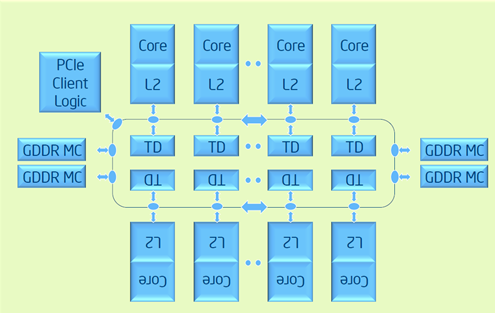
\includegraphics[width=0.6\textwidth]{figures/phi_arch.png}
    \caption{Intel Xeon Phi architecture\cite{opencl_phi}.}
    \label{PhiArch}
\end{figure}

\subsubsection{Mapping}
\begin{itemize}
    \item A \emph{work group} is the smallest task being scheduled on the threads\cite{opencl_phi}.
    \item \emph{Kernels} execute concurrently on multiple \emph{work items} in the SIMD units of every core\cite{opencl_phi_opt}.
    \item Each \emph{work group} is assigned to one thread that loops over all \emph{work items} within the \emph{work group} 
        with SIMD. So you have parallelism at the \emph{work group} level (vector instructions) and parallelism between 
        \emph{work groups} (threading)\cite{opencl_phi_opt}.
    \item At initialization time the Intel OpenCL driver creates 240 software threads and pins them to the hardware threads, then
        when you call \emph{clEnqueueNDRange()}, the intel driver schedules the \emph{work groups} of the current \emph{NDRange}
        into the 240 threads\cite{opencl_phi}.
    \item The OpenCL compiler implicitely vectorize the \emph{work group} routine based on dimension zero loop.
    \item The recommended work-group size for kernels is multiple of 16, which equals the SIMD width for the float and int data 
        type. The automatic vectorization module packs the work-items into SIMD packets of 16 items (for double as well), and 
        processed the rest (“tail”) of the work-group in a scalar way. In other words, a work-group with the size of 2*SIMD\_WIDTH 
        executes faster than, the one with the size of 2* SIMD\_WIDTH-1\cite{opencl_phi_opt,opencl_phi}.
    \item Non-uniform branching at dimension 0 the \emph{NDRange} is executed by flattening the code via predication and 
        ultimatelly executing both path of the branch and then apply masks, thus the usage of non-uniform branching is penalized by 
        a high overhead in the execution of the \emph{kernel}\cite{opencl_phi}.
    \item Using OpenCL \emph{local memory} does not provide any benefit on the Intel Xeon Phi. OpenCL \emph{local memory} is 
        allocated on the regular GDDR memory(\emph{global memory}) and is supported by the cache system like any other memory. 
        Therefore, it introduces additional overhead in terms of redundant data copy and management\cite{opencl_phi}.
    \item The combination of \emph{kernel} with barriers and \emph{work groups} nondivisible by 16, results in the execution of a
        scalar \emph{kernel}.
\end{itemize}

\begin{figure}[!h]
    \centering
    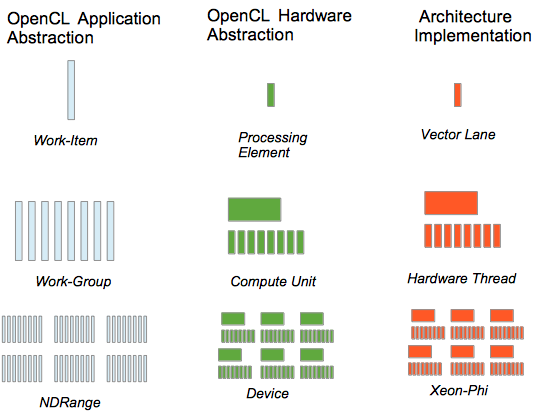
\includegraphics[width=0.7\textwidth]{figures/phi_model.png}
    \caption{OpenCL mapping for Intel Xeon Phi.}
    \label{PhiModel}
\end{figure}

\par{Figure \ref{PhiModel} shows a summary of the mapping of OpenCL concepts into the Intel Xeon Phi co-processor, figure 
    \ref{PhiDeviceInfo} shows the output of an OpenCL information request to the OpenCL run-time, it shows 236 
    \emph{compute units}(one per thread), the size of \emph{local memory} 32KB that match with the total amount of memory for L1 cache and
    the 6GB of total \emph{global memory} that matches with the amount of RAM available on the Intel Xeon Phi. In this context is 
    safe to assume that private memory on the Intel Xeon Phi is implemented via hardware registers.} 

\begin{figure}[!h]
    \centering
    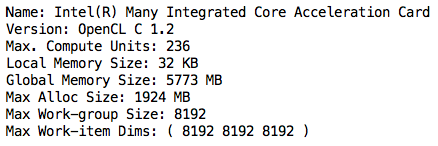
\includegraphics[width=0.7\textwidth]{figures/phi_device_info.png}
    \caption{Intel Xeon Phi device information.}
    \label{PhiDeviceInfo}
\end{figure}




\subsubsection{Two Body Forces}
\par{Two body forces is the code segment that performs the computation of interatomic forces between a pair of atoms. Depending 
on the system that it is computed, Iron or Gramidicin, different contributions are evaluated. If the Iron system is executed, 
metal components of energies and forces are calculated additionally to the computation of Van der Waals and Coulumbic forces and 
energies.}

\par{Two body forces is executed for every time step of the simulation and it was originally implemented sequentially for every MPI 
process. The sequential implementation basically consists of a loop over all the atoms that belong to a MPI process, this loop was 
parallelised with OpenMP obtaining the results shown by the red curve in \fref{fig:mpi1}, this parallelisation forced us to 
introduce one more dimension to several of the arrays used in the code \emph{eg.} forces and distance differences, this way 
avoiding to lose updates due to the multi-threading nature of the parallel implementation. Although we increased the memory 
footprint of the code, with these changes, we were able to parallelise the code improving its performance.}

\par{To improve the performance of our first parallel OpenMP implementation we applied two optimisations. The first one was based 
on \citep{Meloni2003} and consisted of avoding OpenMP reductions over multi-dimensional arrays, writing our own reductions 
for arrays allowed us to improve the performance of the parallel loop. The second improvement was to replace all 
the Fortran allocatable arrays involved in the computation of two body forces by automatic arrays.}

\par{All the procedures called from the parallel region needed an interface, which was implemented by creating Fortran modules
for each file that needed them.}

\par{OpenMP parallelisation achieved very good scalability for Gramidicin, with an efficiency of 87\% for 20 threads on the Host
and 75\% with 60 threads on the Xeon Phi. For Iron the OpenMP parallelisation achieved 78\% efficiency with 20 threads on the 
Host and 62\% efficiency with 60 threads on the Xeon Phi, this is shown by the red curve in \fref{fig:mpi1}. For the Xeon Phi, 
with a thread count over 60 threads the efficiency shows a steep decrease reaching 45\% for Gramidicin and 34\% for Iron. The 
differences in efficiency between Gramidicin and Iron and the poor efficiency of two body forces on the Xeon Phi after 60 threads
on the Xeon Phi need further investigations.}

\par{In terms of absolute times, best cases of the OpenMP parallelisation on the Xeon Phi are 52\% slower for Gramidicin and 97\% 
for Iron than the case when 10 MPI processes are  used on the Host with the original version of the code. The OpenMP 
parallelisation using 20 threads achieved a speedup of 4\% over the MPI base implementation for Gramidicin and its performance 
decreases 18\% for Iron using 20 MPI processes on the Host. Comparing the best executions on the Intel Xeon Phi, the OpenMP 
parallelisations using 120 threads achieved similar results than the MPI only implementation of the code, the OpenMP version 
of the code was 22\% for Iron and 15\% for Gramidicin slower than the MPI original code using 120 MPI processes.}





\subsubsection{Linked Lists}
\par{Verlet neighbour lists, or as they are commonly known linked lists, are a common method in 
molecular dynamics codes to reduce drastically the number of force evaluations
during the time propagation\cite{Verlet1997}. DL\_POLY implements a modern version
of these lists\cite{Pinches1991,Smith1994,Hockney1981}. The main idea is the partitioning of the entire simulation
space into cells such that in order to determine all the atoms with which one atom interacts one needs to check 
only the neighbouring cells. The version implemented in DL\_POLY is efficient with respect to the 
MPI processes, see \fref{fig:base} pink curve, over 70\% for both Gramidicin and Iron on Host. This picture 
is not replicated in the case of the Xeon Phi.}

\par{OpenMP parallelisation of the most time consuming loop involved an extensive refactoring of the original 
implementation. Instead of looping over all the cells and then over all the atoms in a particular cell 
we loop over all the atoms. In this way we increas the amount of work that can be done in parallel. The results, 
presented in \fref{fig:mpi1}, show a good scalability for small thread counts in the case of Iron on both Host 
and Xeon Phi. Unfortunately, not the same behaviour is replicated in the case of Gramidicin. The poor scalability 
can be attributed to the multiple branching within the OpenMP region and the role of the sequential code from this segment.}

\subsubsection{Metal Forces}
\par{This code segment is executed for every time step of the simulation(only in the case of the Iron system) and it is used to 
compute local densities in metals, this is performed using the verlet neighbour list and Finnis-Sinclair type potential 
\citep{finnis1984sen}. These local densities are computed sequentially using two loops over the atoms of every MPI process.}

\par{The parallelisation of this algorithm was performed using OpenMP over these two loops, the results of this parallelisation
are shown by the green curve on the bottom panels of \fref{fig:mpi1}. This parallelisation does not achieve good efficiency, with 
44\% with 20 threads on the Host and 17\% with 60 threads on the Xeon Phi. The main reasons for this poor performance is an 
MPI process synchronization segment at the end of the computation of metal densities and some sequential code still present in
the computation.}

\par{We noticed during the parallelisation of this code that some calculations performed are also computed in 
two body forces \emph{eg.} calculation of the differences between atom positions. To optimise this, we stored these values to not 
perform the same computation twice. We did not obtain good results with this optimisation, due to the increase of memory foot 
print that the implementation of this optimisation introduced, also the code added in two body forces to allow this optimisation 
degraded the performance in the case of the Gramidicin system.}


\subsection{Synchronous Offload Implementation}
\label{sec:offload}
\par{Based on our previous results in Native Mode it is obvious that our OpenMP implementation for MD does not make efficient use
of all the threads available on the Xeon Phi, one way to tackle this issue is to use the co-processor in offload mode. From the 
code segments identified earlier the best candidates for offloading is two body forces due to its good OpenMP scaling on Xeon Phi. 
Shake is the only code segment which due to the MPI synchronization at each iteration is not suitable for offloading, 
Linked Lists and metal local density code segments due to poor OpenMP scalability on the Xeon Phi can be challenging, 
for the rest of this section we will concentrate on the offload of two body forces.}

\par{One can offload data to the co-processor in two ways, using OpenMP 4.0 or Intel LEO (Language Extentions for Offload). As the
code already uses OpenMP for parallelisation is a natural option to use OpenMP also for offloading, unfortunatelly after 
implementing the offload code with OpenMP we discovered an issue with implementation of OpenMP tasks and offload. In order to 
avoid this we changed the offload implementation to Intel LEO. Both, OpenMP and LEO, implementations for the synchronous 
offloading achieved the same performance results.}

\par{One has to upload for each computation to the card: positions, the list of neighbours for each atom and all data related to 
the potential and download from the card to the host the contribution to forces and other statistical quantities.}

\par{In the Gramidicin case when running 1 MPI the data transfered to the Xeon Phi can be as big as 333.54MB and the data 
transfered from the Xeon Phi to the Host \footnote{Intel(R) Xeon(R) CPU E5-2660 v2, 2.20GHz, 64GiB.} is 11.08MB for every time 
step of the simulation, the time spent doing this is 0.24 seconds. By far the biggest chunk of data is associated with 
linked lists.}

\begin{figure}[!ht]
\centering
\begin{tikzpicture}
\centering\tikzstyle{every node}=[font=\tiny]
\begin{groupplot}[
    group style={
        group name=my plots,
        group size=2 by 2,
        xlabels at=edge bottom,
    %    xticklabels at=edge bottom,
        horizontal sep=3mm, vertical sep=0.5cm,
    },
    /tikz/mark size=1.0pt,
    width=0.45\textwidth,
    minor tick num =4,ymin=0,ymax=1.0,
    grid=none,
    legend pos=outer north east,
    legend cell align=left,
    legend style={xshift=5mm},
    every axis label/.append style={font=\footnotesize},
    x tick label style={scaled x ticks = false,
        /pgf/number format/fixed,},
    y tick label style={scaled y ticks = false,
        /pgf/number format/fixed,},
]
\nextgroupplot[ylabel={Time [s]}, xmin=1,xmax=20,ymin=0,ymax=1.4,
 xmode=log, log basis x=2,
 xtick={1,2,4,8,10,16,20},xticklabels={1,2,4,8,10,16,20},ytick={0.0,0.2,0.4,0.6,0.8,1.0,1.2,1.4}]
\addplot +[blue,thick,solid] table[x index=0, y index=  1]  {figures/gram-off-leo-1card-5X.dat};
\addplot +[red,thick,solid] table[x index=0, y index=  2]  {figures/gram-off-leo-1card-5X.dat};
\addplot +[green,thick,solid] table[x index=0, y index=  3]  {figures/gram-off-leo-1card-5X.dat};
\addplot +[pink,thick,solid] table [x index=0, y index=  4] {figures/gram-off-leo-1card-5X.dat};
\nextgroupplot[ylabel={},yticklabel pos=right, ylabel near ticks,xmin=2,xmax=20,
 xmode=log, log basis x=2,
 xtick={2,4,8,10,16,20},xticklabels={2,4,8,10,16,20}]
\addplot +[blue,thick,solid] table [x index=0, y index=  1] {figures/gram-off-leo-2cards-5X.dat};
\addplot +[red,thick,solid] table [x index=0, y index=  2]{figures/gram-off-leo-2cards-5X.dat};
\addplot +[green,thick,solid] table[x index=0, y index=  3] {figures/gram-off-leo-2cards-5X.dat};
\addplot +[pink,thick,solid] table[x index=0, y index=  4] {figures/gram-off-leo-2cards-5X.dat};
\legend{ time per step,
two body forces,
shake,
linked lists}
\nextgroupplot[ylabel={Time [s]}, xlabel={MPI Processes},xmin=1,xmax=24,ymin=0,ymax=1.4,
 xmode=log, log basis x=2,
 xtick={1,2,4,6,8,10,12,16,20,24},xticklabels={1,2,4,6,8,10,12,16,20,24},ytick={0.0,0.2,0.4,0.6,0.8,1.0,1.2,1.4}]
\addplot +[blue,thick,solid] table[x index=0, y index=  1]  {figures/gram-off-leo-1card-7X.dat};
\addplot +[red,thick,solid] table[x index=0, y index=  2]  {figures/gram-off-leo-1card-7X.dat};
\addplot +[green,thick,solid] table[x index=0, y index=  3]  {figures/gram-off-leo-1card-7X.dat};
\addplot +[pink,thick,solid] table [x index=0, y index=  4] {figures/gram-off-leo-1card-7X.dat};
\nextgroupplot[ylabel={},xlabel={MPI Processes},yticklabel pos=right, ylabel near ticks,xmin=2,xmax=24,
 xmode=log, log basis x=2,
 xtick={2,4,6,8,10,12,16,20,24},xticklabels={2,4,6,8,10,12,16,20,24}]
\addplot +[blue,thick,solid] table [x index=0, y index=  1] {figures/gram-off-leo-2cards-7X.dat};
\addplot +[red,thick,solid] table [x index=0, y index=  2]{figures/gram-off-leo-2cards-7X.dat};
\addplot +[green,thick,solid] table[x index=0, y index=  3] {figures/gram-off-leo-2cards-7X.dat};
\addplot +[pink,thick,solid] table[x index=0, y index=  4] {figures/gram-off-leo-2cards-5X.dat};
\end{groupplot}
\node[] at (14.0,3.0) {Xeon Phi 5110P};
\node[] at (14.0,-2.5) {Xeon Phi 7120A};
\end{tikzpicture}
\caption{Best results for DL\_POLY with synchronous offloading for two body forces in the case of Gramidicin, 
upper panels show data for the 5110P model card lower pannels for the 7120A model card vs MPI process count. 
For each case both host and Xeon Phi are saturated with OpenMP threads.
\jref{tab:gramOffLeoMPI15X}, \jref{tab:gramOffLeoMPI25X}, \jref{tab:gramOffLeoMPI17X} 
  and \jref{tab:gramOffLeoMPI27X}}
\label{fig:offleo}
\end{figure}

\par{We carried a systematic study of the offload performance when multiple MPI processes offload the code to one or two cards 
for two body forces the results are presented in \fref{fig:offleo}. Upper panels of \fref{fig:offleo} present results for 
offloading to the 5110P model \footnote{8gb, stepping B1, 1052.630 ghz, 60 cores.} of the Intel Xeon Phi and lower panels show 
the results for the model 7120A \footnote{ 16gb,  C0 stepping, 1.238 ghz, 61 cores, C0QS-7120 (pre-prod 7120A) ivb-ep 12c 
2.5ghz, 128gb.} of the Intel Xeon Phi. The results presented in \fref{fig:offleo} were obtained by running DL\_POLY with a
varying number of MPI processes, when two cards are used for offloading first half of MPI processes offload to card number 0
and the second half to card number 1. For each case when the number of MPI processes was less than the number of cores of the
Host where possible we saturated each MPI process with OpenMP threads. For each MPI process the card was equally partitioned 
and saturated with OpenMP threads. The best results for each MPI process count is selected and presented.}

\par{When we offload to one card, left hand side panel, or two cards, right hand side panel, using more than 4 MPI processes 
offloading to the same card slows down two body forces. This is due to the fact that data transfers dominate over computations, 
hence the need of using a reduced number of MPI processes on Host and an increase of OpenMP threads on the Xeon Phi.}

\par{The best performace for time per step for the 5110P was 0.5~s and 0.42~s for the 7120A card(8 MPI processes) which are slower 
than 0.3~s on the equivalent number of MPI processes on the Host. These results are encouraging as is possible to further improve 
them by using asynchronous computations and data transfers, as we used in a previous work\cite{Elena2014}. Indeed preliminary results were obtained which confirm this and will
be presented in a further communication.} 



\subsection{MPI Native and Symmetric}
\label{sec:mpis}
\par{Another way in which one can exploit the Intel Xeon Phi is MPI symmetric mode. Unfortunatelly the results we obtained by 
executing DL\_POLY in symmetric mode were on the same level of performance with MPI native results. This was expected because of 
the nature of the calculation, for each time step a MPI collective synchronization is performed hence the slowest component 
dominates the timings. At the moment data distribution over MPI processes is homogeneous, an heterogeneous distribution should be 
implemented if one wants to exploit this execution model.}


\section{Future Work and Conclusions}
\par{We successfully ported DL\_POLY to Xeon Phi and showed that without an intensive effort into optimisation it is 
difficult to fully take advantage of the Xeon Phi co-processor. Moderate success can be claimed for the OpenMP implementation were
we showed that for intensive routines with the right type of parallelism in native mode we can be as fast as the host, 
\emph{eg.} Shake. MPI symmetric seems to be a no go area as long as the homogenous decomposition of data is maintained.
By far the most promising is the offload mode, where synchronous offloading showed encouraging results. Future work will 
concentrate on mixing asynchronous computation and data transfers as promising sources of speed-up.}

%------------------------------------------------
\phantomsection
\section*{Acknowledgments} % The \section*{} command stops section numbering
\addcontentsline{toc}{section}{Acknowledgments} % Adds this section to the table of contents with negative horizontal space equal to the indent for the numbered sections
\par{to be added}


%----------------------------------------------------------------------------------------
%	REFERENCE LIST
%----------------------------------------------------------------------------------------
\phantomsection
\bibliographystyle{unsrt}
\bibliography{report}

\phantomsection
\section*{Supplementary Information} % The \section*{} command stops section numbering
\addcontentsline{toc}{section}{Supplementary Information} % Adds this section to the table of contents with negative horizontal space equal to the indent for the numbered sections
\par{...}

%----------------------------------------------------------------------------------------

\end{document}
